\documentclass[11pt, a4paper, twoside]{article}   	% use "amsart" instead of "article" for AMSLaTeX format

\usepackage{geometry}                		% See geometry.pdf to learn the layout options. There are lots.
\usepackage{pdfpages}
\usepackage{caption}
\usepackage{minted}
\usepackage[german]{babel}			% this end the next are needed for german umlaute
\usepackage[utf8]{inputenc}
\usepackage{color}
\usepackage{graphicx}
\usepackage{titlesec}
\usepackage{fancyhdr}
\usepackage{lastpage}
\usepackage{hyperref}
\usepackage[autostyle=false, style=english]{csquotes}
\usepackage{mathtools}
\usepackage{tabularx}
% http://www.artofproblemsolving.com/wiki/index.php/LaTeX:Symbols#Operators
% =============================================
% Layout & Colors
% =============================================
\geometry{
   a4paper,
   total={210mm,297mm},
   left=20mm,
   right=20mm,
   top=20mm,
   bottom=30mm
 }	

\definecolor{myred}{rgb}{0.8,0,0}
\definecolor{mygreen}{rgb}{0,0.6,0}
\definecolor{mygray}{rgb}{0.5,0.5,0.5}
\definecolor{mymauve}{rgb}{0.58,0,0.82}

\setcounter{secnumdepth}{4}


% the default java directory structure and the main packages
\newcommand{\srcEmit}{../src/Reflection.Emit.Solution/Reflection.Emit}
\newcommand{\srcSymbolic}{../src/Reflection.Emit.Solution/Symbolic.Computation}
\newcommand{\imageDir}{images}
% =============================================
% Code Settings
% =============================================
\newenvironment{code}{\captionsetup{type=listing}}{}
\newmintedfile[cppSourceFile]{cpp}{
	linenos=true, 
	frame=single, 
	breaklines=true, 
	tabsize=2,
	numbersep=5pt,
	xleftmargin=10pt,
	baselinestretch=1,
	fontsize=\footnotesize
}

\newcommand{\xvdash}[1]{%
  \vdash^{\mkern-10mu\scriptscriptstyle\rule[-.9ex]{0pt}{0pt}#1}%
}

% =============================================
% Page Style, Footers & Headers, Title
% =============================================
\title{Übung 3}
\author{Thomas Herzog}

\lhead{Übung 3}
\chead{}
\rhead{
\includegraphics[scale=0.10]{FHO_Logo_Students.jpg}}

\lfoot{S1610454013}
\cfoot{}
\rfoot{ \thepage / \pageref{LastPage} }
\renewcommand{\footrulewidth}{0.4pt}
% =============================================
% D O C U M E N T     C O N T E N T
% =============================================
% =============================================
% 2016.10.13: 1 
% 2016.10.14: 2
% =============================================
\pagestyle{fancy}
\begin{document}
\setlength{\headheight}{15mm}
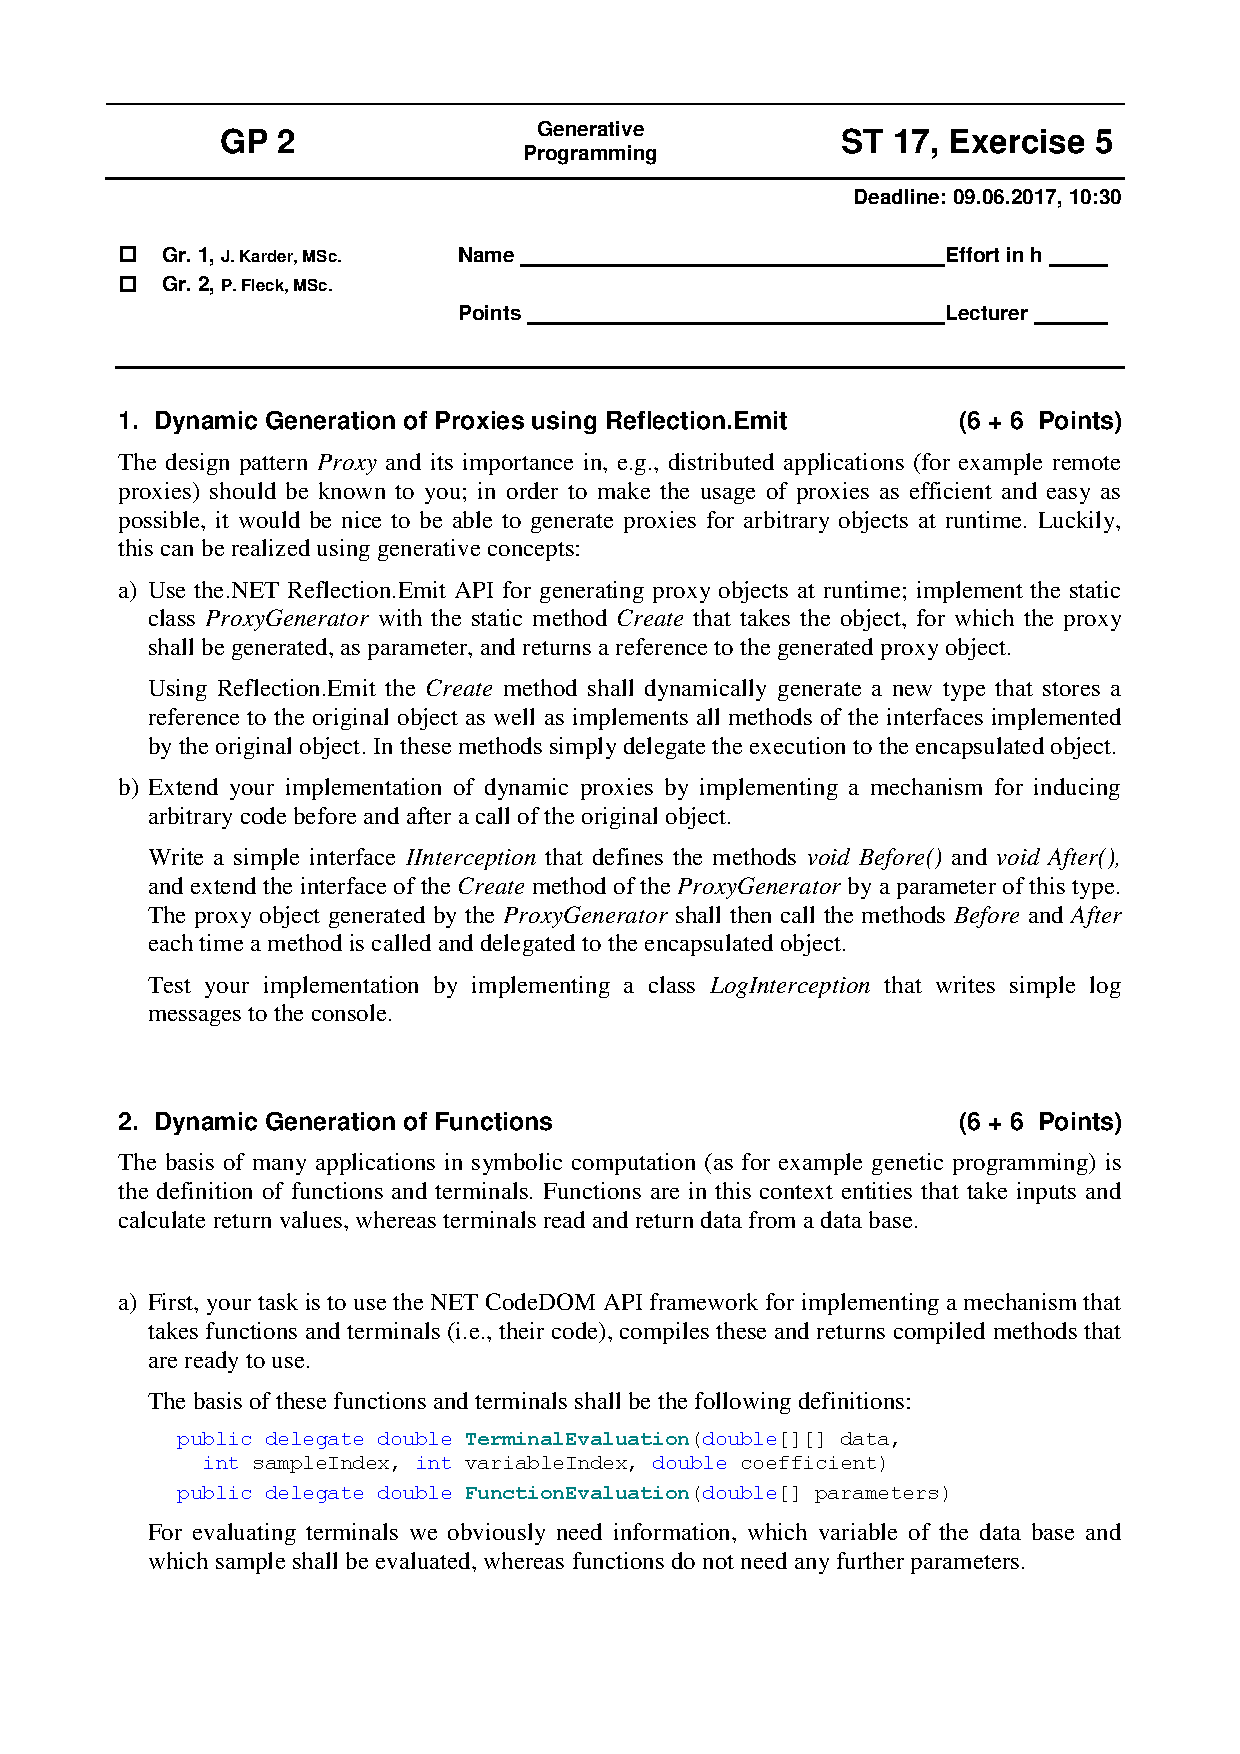
\includepdf[pages={1,2}]{GP_A05.pdf}

\section{Dynamic Generation of Proxies using Reflection.Emit}
Dieser Abschnitt behandelt die Aufgabenstellung \emph{Dynamic Generation of Proxies using Reflection.Emit}.

\subsection{Lösungsidee} 
Es wird die Klasse \emph{ProxyGenerator} implementiert, welche die beiden generischen Methoden \emph{Create$<T>$(T obj)} und \emph{Create$<T>$(T obj, IInterception$<T>$ interceptor)} zur Verfügung stellt, die für das übergebene Objekt eine Proxyklasse erstellen und das Proxyobjekt zurückliefern. Damit der Proxy auch bei einem \emph{Cast} auf den implementierten Typ greift, müssen die implementierten Methoden als \emph{virtual} markiert werden, ansonsten wird die Implementierung des konkreten Typs verwendet und nicht die überschriebenen Methoden des Proxy, was an der Art und Weise der Handhabung von der Methodenbindung in C\# liegt.
\newline
\newline
Es werden alle Methoden im Proxy überschrieben, jedoch wird der \emph{Interceptor} nur bei den Methoden, die im Typ \emph{T} zur Verfügung stehen eingefügt. Ein Interceptor wird durch die Schnittstelle \emph{IIntercepton} spezifiziert wobei die beiden Methoden \emph{Before} und \emph{After} für einen \emph{Interceptor} zur Verfügung stehen. Diese beiden Methoden \emph{Before} und \emph{After} bekommen das Objekt und den Methodennamen übergeben, sodass der \emph{Interceptor} mit dem Objekt interagieren kann und auch die Information hat welche Methode aufgerufen wird.
\newline
\newline
Es wird die Klasse \emph{LogInterception} implementiert, welche die Schnittstelle \emph{IInterception} implementiert und bei einem Aufruf der Methoden \emph{Before} und \emph{After} \emph{Logs} generiert.

\subsection{Quelltexte}
Dieser Abschnitt beinhaltet die implementierten Quelltexte und das Testprogramm.
\begin{code}
	\caption{IInterception.cs}
	\cppSourceFile{\srcEmit/IInterception.cs}
	\label{src:interface-iinterception}
\end{code}

\begin{code}
	\caption{Interfaces.cs}
	\cppSourceFile{\srcEmit/Interfaces.cs}
	\label{src:interface-itest-isecondtest}
\end{code}

\begin{code}
	\caption{LogInterception.cs}
	\cppSourceFile{\srcEmit/LogInterception.cs}
	\label{src:class-loginterception}
\end{code}

\begin{code}
	\caption{Test.cs}
	\cppSourceFile{\srcEmit/Test.cs}
	\label{src:class-test}
\end{code}

\begin{code}
	\caption{ProxyGenerator.cs}
	\cppSourceFile{\srcEmit/ProxyGenerator.cs}
	\label{src:class-proxagenerator}
\end{code}

\begin{code}
	\caption{Program.cs}
	\cppSourceFile{\srcEmit/Program.cs}
	\label{src:class-program}
\end{code}

\subsection{Tests}
Dieser Abschnitt behandelt die Tests in Form von Ausgaben der \emph{Logs}.
\begin{figure}[h]
	\centering
	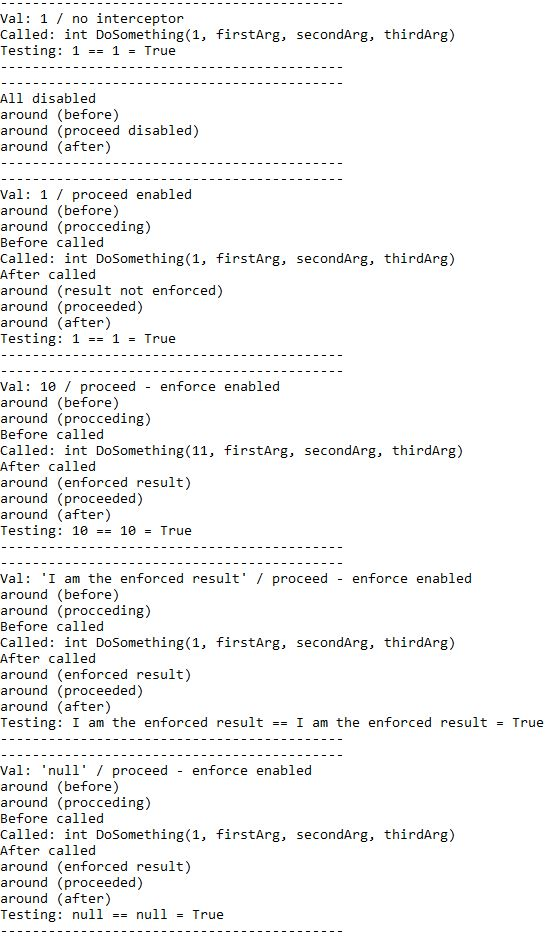
\includegraphics[scale=0.75]{\imageDir/test-proxy-generator.JPG}
	\caption{Test für \emph{Interception} von \emph{ITest} und \emph{ISecondTest}}
	\label{fig:image-proxy-generator}
\end{figure}

\ \newpage
\begin{figure}[h]
	\centering
	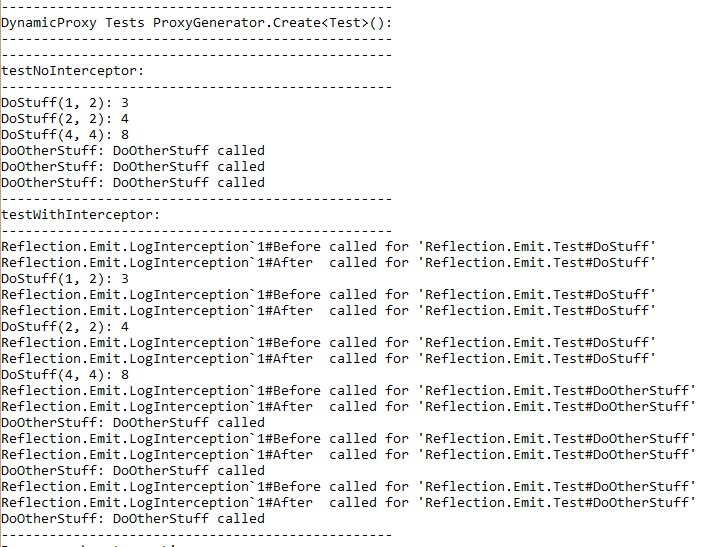
\includegraphics[scale=0.75]{\imageDir/test-proxy-generator-2.JPG}
	\caption{Test für \emph{Interception} von \emph{Test}}
	\label{fig:image-proxy-generator-2}
\end{figure}
\ \newpage

\section{Dynamic Generation of Functions}
Dieser Abschnitt behandelt die Aufgabenstellung \emph{Dynamic Generation of Functions}.

\subsection{Lösungsidee}
Ein Großteil der Implementierungen wurde bereits in der Übung implementiert, jedocjh wurden folgende Veränderungen vorgenommen. Die Methode \emph{CompileTerminal} bekommt die Argumente als String Array übergeben, sodass beim Erstellen der Aufrufer nicht von statischen Definitionen dieser Implementierung abhängig ist, die bereits vorgeben, wie die Argumente der erstellten Methode benannt sind. Ebenso wird dieser Methode der Datentyp des Resultats dieser Methode übergeben.
\newline
\newline
Die Methode \emph{CompileFunction} bekommt ebenfalls das Argument in Form eines Strings und den Datentyp des Resultats dieser Methode übergeben, damit auch bei dieser Methode der Aufrufer nicht abhängig ist von statische Definitionen der Implementierung, die bereits den Namen und Datentyp des Resultats definieren.
\newline
\newline
Es wird die Schnittstelle \emph{INode} implementiert, die eine Node im Evaluierungsbaum darstellt. Es wird die abstrakte Klasse \emph{BaseNode} implementiert, die alle gemeinsamen \emph{Properties} kapselt. Es werden die Klassen \emph{FunctionalNode} und \emph{TerminalNode} implementiert, welche die Knoten der zwei Typen von Evaluierungsmethoden repräsentieren und die spezifischen Evaluierungen dieser Knotentypen implementieren. 

\subsection{Quelltexte}
Dieser Abschnitt beinhaltet die implementierten Quelltexte und das Testprogramm.
\begin{code}
	\caption{AssertDouble.cs}
	\cppSourceFile{\srcSymbolic/AssertDouble.cs}
	\label{src:class-assertdouble}
\end{code}
\ \newpage
\begin{code}
	\caption{Node.cs}
	\cppSourceFile{\srcSymbolic/Node.cs}
	\label{src:class-inode-basenode-functional-node-terminal-node}
\end{code}

\begin{code}
	\caption{FunctionalBasis.cs}
	\cppSourceFile{\srcSymbolic/FunctionalBasis.cs}
	\label{src:class-functional-basis}
\end{code}

\begin{code}
	\caption{Program.cs}
	\cppSourceFile{\srcSymbolic/Program.cs}
	\label{src:class-symbolic-program}
\end{code}

\subsection{Tests}
Dieser Abschnitt beinhaltet die implementierten Quelltexte und das Testprogramm.
\begin{figure}[h]
	\centering
	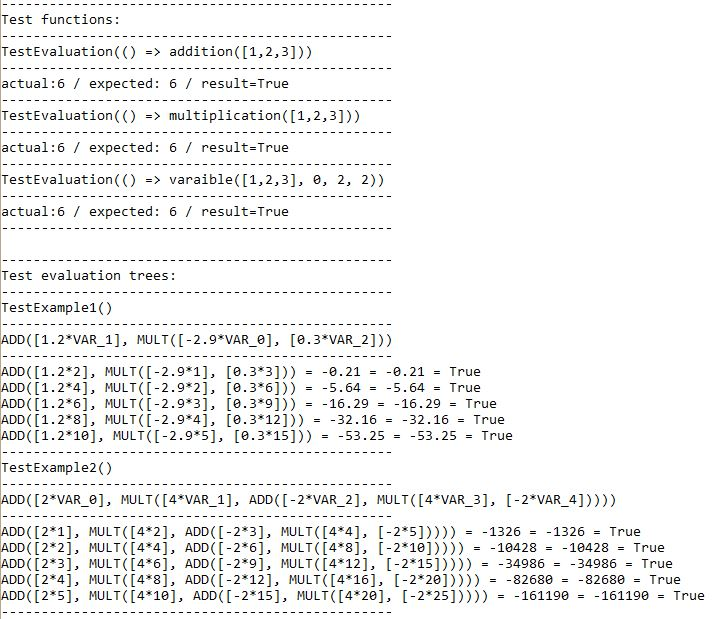
\includegraphics[scale=0.8]{\imageDir/test-symbolic-compuation.JPG}
	\caption{Ausgabe des Testprogramms}
	\label{fig:test-symbolic-compuation}
\end{figure}

\end{document}